\documentclass[tikz]{standalone}

\usepackage{amssymb}
\usetikzlibrary{calc}
\usetikzlibrary{shapes.geometric}
\usetikzlibrary{decorations.markings}
\begin{document}
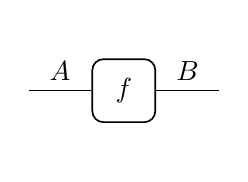
\begin{tikzpicture}[unit length/.code={{\newdimen\tikzunit}\setlength{\tikzunit}{#1}},unit length=4mm,x=\tikzunit,y=\tikzunit,semithick,box/.style={rectangle,draw,solid,rounded corners},outer box/.style={draw=none},wire/.style={draw,postaction={decorate},decoration={markings,mark=at position 0.5 with {#1}}}]
\node[outer box,minimum width=6\tikzunit,minimum height=4\tikzunit] (root) at (0,0) {};\node[box,minimum size=2\tikzunit] (n1) at (0,0) {$f$};\path[wire={\node[anchor=south] {$A$};}] (root.west) to[out=0,in=-180] (n1.west);\path[wire={\node[anchor=south] {$B$};}] (n1.east) to[out=0,in=180] (root.east);
\end{tikzpicture}
\end{document}
